\label{sec:rnn_results}
This study focuses on one particular type of model which has proved to be very effective in text classification and prediction, a recurrent neural network utilizing long short-term memory (LSTM) units.  Our base model has one layer of LSTM units where the output of each unit is averaged over time followed by a fully connected layer with two outputs, and a softmax function.  The output represents the neural network's confidence in its prediction.

The model was trained for 50 epochs over the entire training set with a batch size of 1000 and a maximum unfolding length of 1024, meaning that 27 reviews would be clipped.  The Adam optimizer with exponential step decay factor of 0.8 every 500 batches was used to minimize the model loss, softmax cross entropy.  We used forget gates, peepholes, and output dropout for training.  

We trained fourteen models, varying the number of hidden units and initial learning rates.  The final training and testing accuracies are shown in tables \ref{tab:train_accuracy} and \ref{tab:test_accuracy} respectively.  As expected, increasing the model size always increased the training accuracy, as did increasing the learning rate.  The testing accuracy was less predictable.  Most accuracies were in the neighborhood of 80\%, 30\% greater than the baseline of 50\% random guessing.

\begin{table}
\centering
\begin{tabular}{ |c|c|c|c|c|c|c|}
    \hline
    \multicolumn{7}{|c|}{Number of Hidden Units, Learning Rate = 0.01}\\ \hline
    2 & 4 & 8 & 16 & 32 & 64 & 128 \\ \hline
    0.778 & 0.784 & 0.812 & 0.850 & 0.878 & 0.904 & 0.961 \\ \hline
    \multicolumn{7}{|c|}{Number of Hidden Units, Learning Rate = 0.1}\\ \hline
    2 & 4 & 8 & 16 & 32 & 64 & 128 \\ \hline
    0.827 & 0.853 & 0.895 & 0.965 & 0.975 & 0.997 & 0.990 \\ \hline
\end{tabular}
\caption{Training Accuracy}
\label{tab:train_accuracy}
\end{table}

\begin{table}
\centering
\begin{tabular}{ |c|c|c|c|c|c|c|}
    \hline
    \multicolumn{7}{|c|}{Number of Hidden Units, Learning Rate = 0.01}\\ \hline
    2 & 4 & 8 & 16 & 32 & 64 & 128 \\ \hline
    0.753 & 0.755 & 0.771 & 0.809 & 0.816 & 0.829 & 0.834 \\ \hline
    \multicolumn{7}{|c|}{Number of Hidden Units, Learning Rate = 0.1}\\ \hline
    2 & 4 & 8 & 16 & 32 & 64 & 128 \\ \hline
    0.793 & 0.816 & 0.827 & 0.822 & 0.815 & 0.809 & 0.817 \\ \hline
\end{tabular}
\caption{Testing Accuracy}
\label{tab:test_accuracy}
\end{table}

The average training and test losses of each model are given in figures \ref{fig:train_curve} and \ref{fig:test_curve}.  The spacing on the training curve is finer because the value was sampled every epoch instead of every five epochs as in the case of the testing accuracy.


\begin{figure}
    \centering
    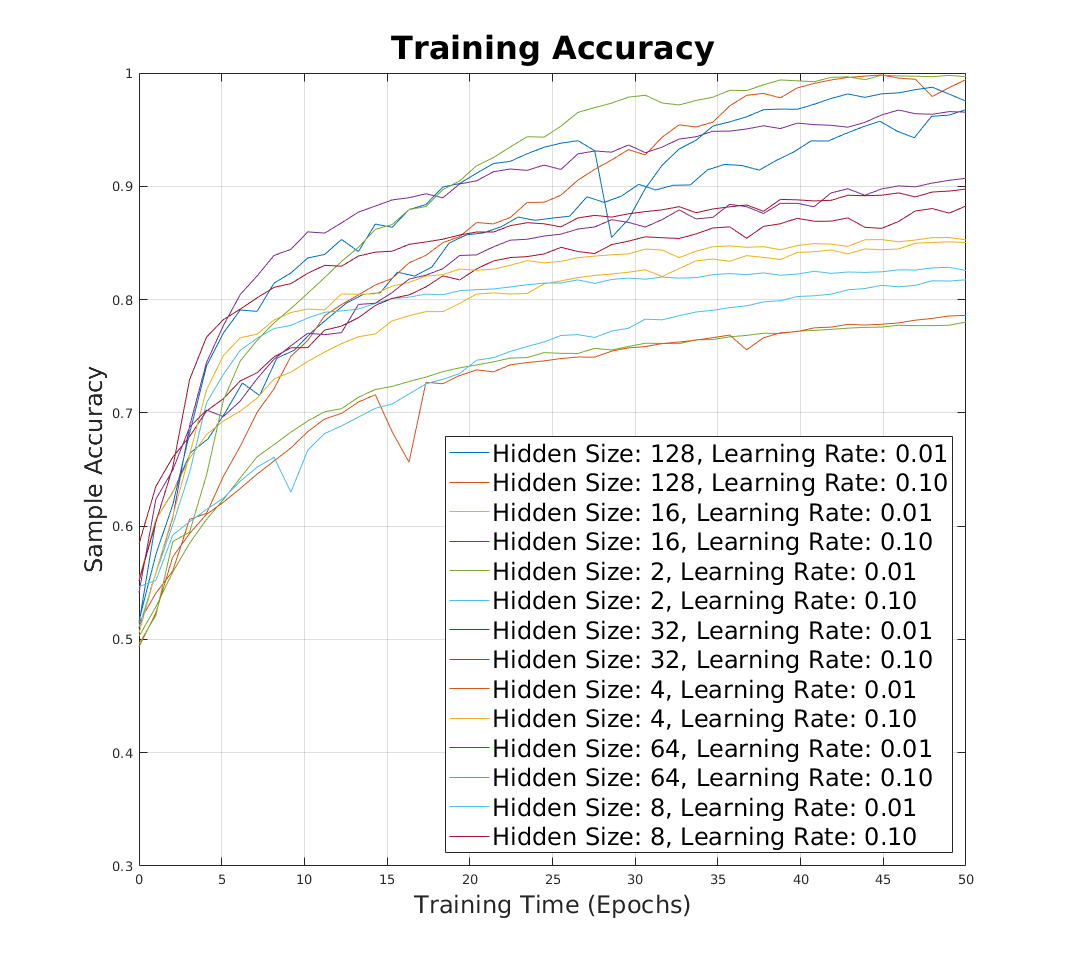
\includegraphics[width=\textwidth]{train_curve.png}
    \caption{Training Accuracy of RNNs}
    \label{fig:test_curve}
\end{figure}

\begin{figure}
    \centering
    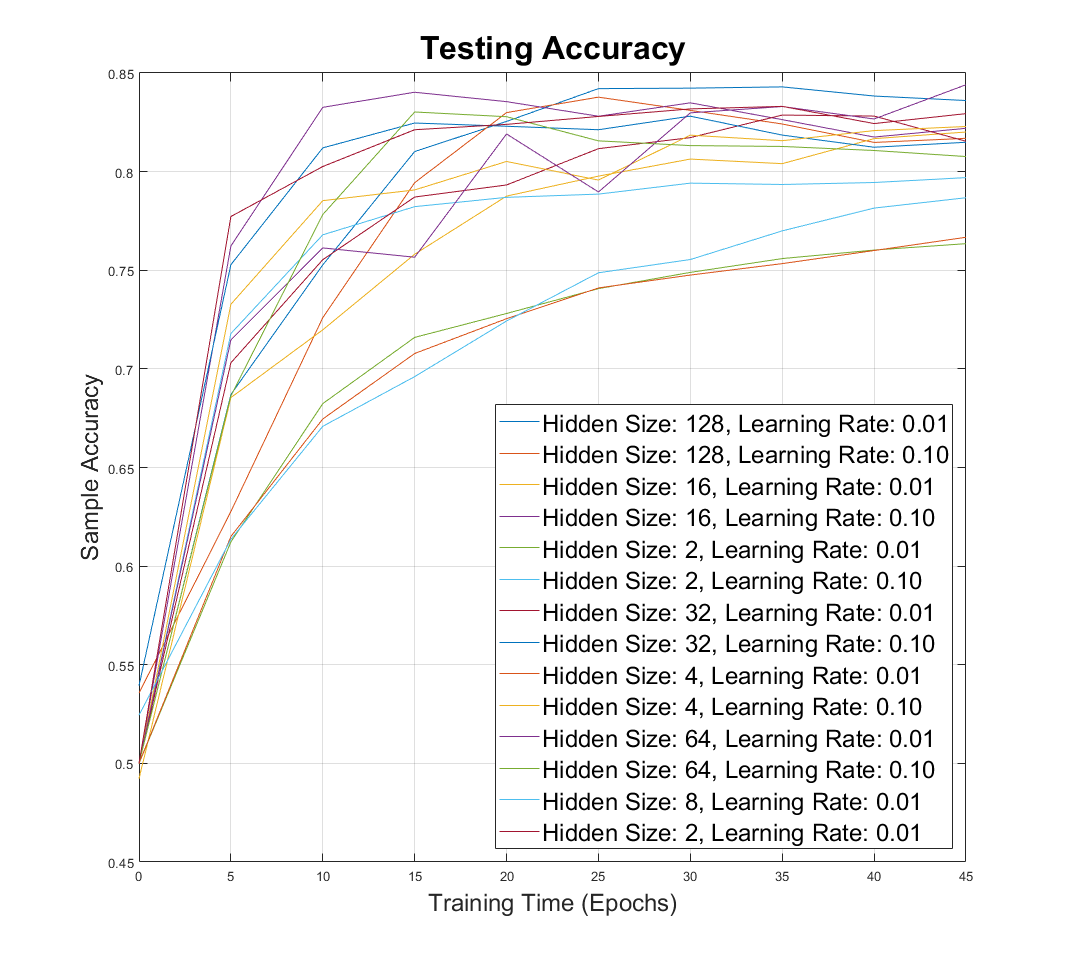
\includegraphics[width=\textwidth]{test_curve.png}
    \caption{Testing Accuracy of RNNs}
    \label{fig:train_curve}
\end{figure}
